
\section{Preprocessing and performance}
\label{sec:exp_preprocessing}

We assume the light curves segments are obtained from a median normalized light curve, e.g. by splitting the original light curve into equally sized parts. Assuming for now that no gaps are present in these segments, several additional preprocessing steps can be considered. One approach is to center the segments around zero by subtracting 1 from the flux values, and doing nothing else. Additionally, one could scale the light curves by their estimated noise level $\sigma$, so the network performance becomes less dependent on this noise and instead more on the transit depth relative to this noise. We refer to the latter step as sigma scaling, and adopt this in following experiments.  See figures \ref{fig:preprocessing-scaling_lcsim} and \ref{fig:preprocessing-scaling_lilith} for the effect of these basic preprocessing steps on the performance of the network during training. \todo{mention that each all data is standardized as last preprocessing step}

\begin{figure}
    \centering
    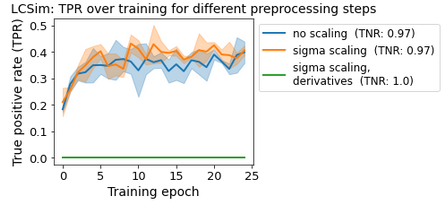
\includegraphics[width=0.5\linewidth]{Experiments/Figures/Preprocessing/preprocessing_lcsim_valid.png}
    \caption{\todo{caption}}
    \label{fig:preprocessing-scaling_lcsim}
\end{figure}

\begin{figure}
    \centering
    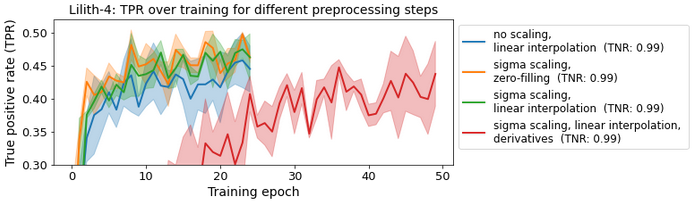
\includegraphics[width=0.75\linewidth]{Experiments/Figures/Preprocessing/preprocessing_lilith_valid_2.png}
    \caption{\todo{caption}}
    \label{fig:preprocessing-scaling_lilith}
\end{figure}

In both cases however, the range of flux values might still greatly vary between two separate light curve segments. This is understood by realizing that the original light curve may contain large-scale fluctuations due to stellar rotation modulation. The network might interpret these range differences as indicators of the presence of a transit signal, in particular if there is little data available for a certain range of flux values. This is not what we want, because a transit event can occur at any given time, independent from the activity on the stellar surface. This potential problem is visualized in Figure \ref{fig:preprocessing-ranges}.

\begin{figure}
    \centering
    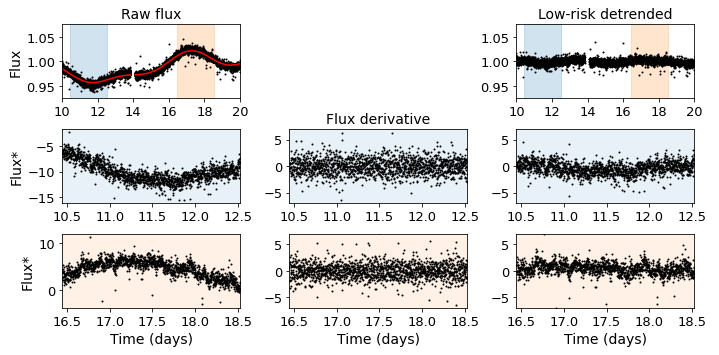
\includegraphics[width=0.8\linewidth]{Experiments/Figures/Preprocessing/prepocessing_ranges_example.png}
    \caption{\todo{caption}}
    \label{fig:preprocessing-ranges}
\end{figure}

We consider two approaches to resolve this issue: (i) feed the differences between flux values to the network, instead of their absolute values, and (ii) remove large-scale patterns from the original light curve, a process we will refer to as low-risk detrending (LRD). Both approaches have the desired effect of making the input ranges more consistent, with some exceptions. The benefits of (i) are that this approach can be applied to the segments directly and we lose almost no information by doing so. However, although all the information is still there, the structure of the data is completely changed which might be difficult for the network to learn. For (ii), we need to alter the original light curve prior to splitting it into segments. By doing so we lose information, but the result is more intuitive than (i).

In Figure \ref{fig:preprocessing-general_lilith} we compare the effect of several different preprocessing steps on the performance of the network trained on Lilith-4 data. In addition to the ``basic preprocessing'' and the ``low-risk detrending'' as described above, several other approaches are included in the comparison. For example, ``high-risk detrending'' means the input light curves are detrended such that both large and short-scale patterns are removed. This is referred to as high-risk as it comes with more risk of partly removing transit signals. The detrending filter we use for this is a time-windowed median filter with a window of 12 hours. Since real-world data may include outliers, we also evaluate the effect of removing these from the data. Outliers are identified after the light curve is detrended with a time-windowed median filter with a window of 30 minutes. Positive outliers at more than 6 standard deviations from the median and negative outliers at more than 12 standard deviations from the median are removed from the original light curve. The detrending step and the low negative-outlier threshold are to avoid transit signals from being flagged s outlier. Lastly, since Lilith-4 provides centroid data, which we also have access to for real-world data, we test the effect of using these as additional input to the network. This means that the network input at each time step consists of three values: the flux, and two values that specify the pointing of the telescope at that time step. Before use, we center the centroid data around zero, and scale them similarly to their corresponding light curve. Subsequently all the centroids in the data set are standardized independently from the flux values. This way of preprocessing is to ensure that the relative scale between light curves and their corresponding centroid data is not altered, as this might contain relevant info for the network. The series of centroid data are split into segments together with their corresponding light curve.

The results show that outlier removal had a negative influence on the performance of the network. This was unexpected, because outliers are not expected to carry relevant information. After all, an outlier should be present regardless of whether a transit event is occurring, unless the transit itself is flagged as outlier. This is unlikely to be the case, as we observe worse performance for both deep and shallow transits. We expect therefore that the reason for this result lies in the fact that outlier removal creates missing data. Missing values were imputed for this experiment, which might have caused the network to perform worse in this case. All other preprocessing steps seem to produce similar results. This is noteworthy, as the network therefore does not have to rely high-risk detrended data, as opposed to other common detection methods. 

Lastly, since Figure \ref{fig:preprocessing-general_lilith} does not clearly indicate whether or not using centroid data is beneficial, we take into consideration the results obtained on the validation set created from Lilith-4. These results, shown in Figure \ref{fig:preprocessing-general_lilith_valid}, do indicate a potential benefit of including the centroids as input to the network. This motivated us to adopt LRD as standard preprocessing procedure in combination with using centroid inputs when applying our network to Lilith-4 data in following experiments. 

\begin{figure}
    \centering
    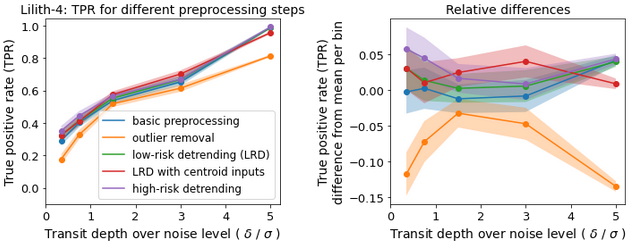
\includegraphics[width=0.65\linewidth]{Experiments/Figures/Preprocessing/test_lilith_pp.png}
    \caption{\todo{caption}}
    \label{fig:preprocessing-general_lilith}
\end{figure}

\begin{figure}
    \centering
    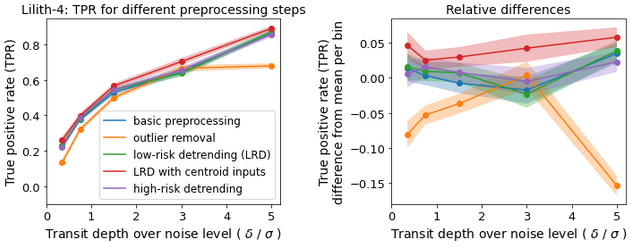
\includegraphics[width=0.65\linewidth]{Experiments/Figures/Preprocessing/validation_lilith_pp.png}
    \caption{\todo{caption}}
    \label{fig:preprocessing-general_lilith_valid}
\end{figure}

Lastly, we address the problem of missing data in greater depth. Lilith-4 data already contains data gaps, which we filled by linear interpolation up to this point, unless stated otherwise. For LCSim light curves, we manually inject NaN values in the pre-generated light curve segments to simulate data gaps. For each data split, 35\% of the samples was injected with one large data gap ranging from 2 to 10 hours, and 15\% was injected with two large data gaps. Apart from the larger gaps, each data point was replaced by a NaN value with 2\% probability. 

Three different approaches to handling gaps are evaluated. In each of the approaches, we impute the data in a different way. First, we consider replacing all missing values with zeros in the centered light curve segment. This is equivalent to replacing missing values with ones in the non-centered light curve. In the second approach, we fill the gaps by linear interpolation. When doing this, we linearly interpolate the trend of the light curve, rather than the raw flux values at the edges of a gap. The reason why we do not use the raw flux instead, is that an extreme value or outlier next to a gap could result in an apparent jump in the flux over consecutive points if it is used for interpolation. Lastly, we use the generative network as described in Section \ref{sec:extension_gen} to fill in gaps as it steps through the light curve. An example of each of the approaches is visualized in Figure \ref{fig:preprocessing-gap_examples}. 

\begin{figure}
    \centering
    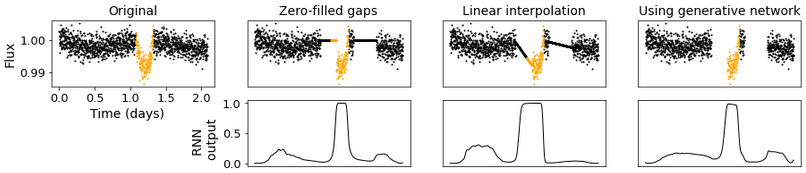
\includegraphics[width=0.8\linewidth]{Experiments/Figures/Preprocessing/gaps_example.png}
    \caption{\todo{caption}}
    \label{fig:preprocessing-gap_examples}
\end{figure}

The generative network seems to work as intended by inspecting Figure \ref{fig:preprocessing-gap_examples}. We can take a closer look at what this network is doing in Figure \ref{fig:preprocessing-generative_example}. The network is bidirectional, so we get two streams of predictions. We can see that these can complement each other. If we only consider the predictions from left-to-right in the first gap and from right-to-left in the second, then the missing values are well reconstructed. However, since each unidirectional component of the network has no information of what comes after a gap, we see the predictions drift off to unrealistic values.

\begin{figure}
    \centering
    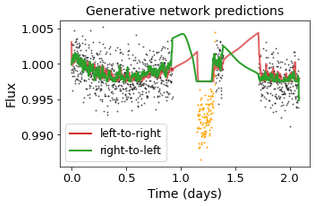
\includegraphics[width=0.34\linewidth]{Experiments/Figures/Preprocessing/generative_example.png}
    \caption{\todo{caption}}
    \label{fig:preprocessing-generative_example}
\end{figure}

After evaluation on the gap-injected test set, of which the results are presented in Figure \ref{fig:preprocessing-gaps_lcsim}, we find that each approach to handling gaps leads to similar network performance in terms of TPR, at the same value for TNR. However, on average linear interpolation seems to work slightly better than the other approaches, which we therefore use in following experiments.

\begin{figure}
    \centering
    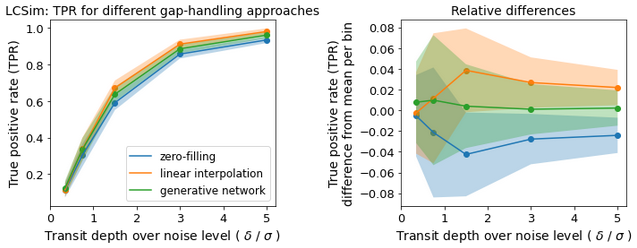
\includegraphics[width=0.65\linewidth]{Experiments/Figures/Preprocessing/pp_gaps_lcsim.png}
    \caption{\todo{caption}}
    \label{fig:preprocessing-gaps_lcsim}
\end{figure}